\chapter*{Introduction}
\section*{Latent variable model}
A latent variable model is a statistical model that relates a set of observable variables (so-called manifest variables) to a set of latent variables.
\\ The motivation behind latent variable modeling is to capture complex or conceptual properties of a system that are difficult to quantify or measure directly. For example we can think of a random process that generates millions of pixel-images of dogs. If we want to learn this random process and generate our own images, it will be a difficult task to generate the multitudes of pixels that form these pictures. However, if we think of that random process as the conceptually simpler process of : first choosing a breed of a dog and only after that sampling a picture with the same dog breed, this may lead us to a better model. VAEs strive to create disentangled latent representations that allow choose characteristic such as dog breed. \\ 
Let's denote $X$ as observed data and $z$ as latent variables of the data. \\ Using Bayesian statistics,  we can look at the distribution of z as the prior, and the distribution of $z|X$ as posterior. We assume that the data ($X$) is i.i.d. relative to $P_{data}$. \\ 
Using this modeling, we seek parameters $\theta$ that maximize the log-likelihood of our data:
\begin{gather*}
\theta = \underset{\theta}{\arg\max} \ log \ p_{\theta}(X)=\underset{\theta}{\arg\max} \sum_{i=1}^{n} log \ p_{\theta}(X^{(i)})=\underset{\theta}{\arg\max} \sum_{i=1}^{n}log \int_z p_{\theta}(X^{(i)}|z)p_{Z}(z)dz
\end{gather*}
In most scenarios, the above optimization problem is hard to compute or intractable. To overcome This problem, we can use Monte-Carlo estimator for this integral and just sample from our prior $p_{Z}$ and leading to the following optimization problem: 
\begin{gather*}
\theta = \underset{\theta}{\arg\max} \sum_{i=1}^{n}log \frac{1}{K} \sum_{k=1}^{K} p_{\theta}(X^{(i)}|z_{k}^{(i)})p_{Z}(z_{k}^{(i)}) \quad , when \ z^{k}\sim p_{Z}
\end{gather*}
The main problem with prior sampling as suggested is that is not very informative. If we look at z as a continuous distribution, the sampled z's will most likely to cause $p_{\theta}(X^{(i)}|z^{k})$ to be equal to zero, and thus the $\theta$ parameters that we will get from the problem will not be very informative. \\ That problem lead to the development of importance sampling and the variational inference approach as follows: 
\begin{gather*}
\theta=\underset{\theta}{\arg\max} \sum_{i=1}^{n}log \int_z p_{\theta}(X^{(i)}|z)p_{Z}(z)dz = \underset{\theta}{\arg\max} \sum_{i=1}^{n}log \int_z \frac{q_{\Phi}(z)}{q_{\Phi}(z)}p_{\theta}(X^{(i)}|z)p_{Z}(z)dz= \\ \\ = \underset{\theta}{\arg\max} \sum_{i=1}^{n}log \mathbb{E}_{z \sim q_{\Phi}(z)}[\frac{p_{\theta}(X^{(i)}|z)}{q_{\Phi}(z)}p_{Z}(z)] \approx \underset{\theta}{\arg\max} \sum_{i=1}^{n}log \sum_{k=1}^{K}\frac{p_{\theta}(X^{(i)}|z_{k}^{(i)})}{q_{\Phi}(z_{k}^{(i)})}p_{Z}(z_{k}^{(i)}) \\ \\ , when\ z^{k}\sim q_{\Phi} \ and \ q_{\Phi} \ is \ some \ distribution \ with \ parameters \ \Phi.
\end{gather*}
We can see that a good-informative approximation to $q_{\Phi}(z)$ will be the posterior of z (i.e $z|X^{(i)}$). To achieve a good approximation of $q_{\Phi}(z)$ we'll use KL-diverge and the objective will be: 
\begin{gather*}
\underset{\theta,\Phi}{\arg\max} \sum_{i=1}^{n}log \sum_{k=1}^{K}\frac{p_{\theta}(X^{(i)}|z_{k}^{(i)})}{q_{\Phi}(z_{k}^{(i)})}p_{Z}(z_{k}^{(i)}) - KL(q_{\Phi}(z)||p_{\theta}(z|X))
\end{gather*}
Another derivation to this objection is from Variational Bayesian method.\\
Let us find a good approximation to some posterior\\ \\
\begin{gather*}
KL(q(z)||p(z|X))=\mathbb{E}_{z \sim q(z)}[log \ q(z)-log \ p(z|X)] = \\  
= \mathbb{E}_{z \sim q(z)}[log \ q(z) - log \ \frac{p(z,X)}{p(X)}] = \\ 
=(1) \mathbb{E}_{z \sim q(z)}[log \ q(z) - log \ p(z) - log \ p(X|z)] + log \ p(X) \\ 
\end{gather*}
According to (1), if we want to maximize the log-likelihood we need to maximize : \\ \\
$log \ p(X) = \underbrace{\mathbb{E}_{z \sim q(z)}[-log \ q(z) + log \ p(z) + log \ p(X|z)]}_{ELBO}+KL(q(z)||p(z|X))$ \\ \\
The Evidence lower bound (ELBO) appropriately lower bounds the above term because KL is lways positive. Thereby, the following inequality: \\ \\
$log \ p(X) = \underbrace{\mathbb{E}_{z \sim q(z)}[-log \ q(z) + log \ p(z) + log \ p(X|z)]}_{ELBO}+KL(q(z)||p(z|X)) \underbrace{\geq}_{KL \geq 0} ELBO $ \\
\section*{ELBO Maximization}
We maximize ELBO and not ($\mathbb{E}_{z \sim q_{\Phi}(z)}[-log \ q_{\Phi}(z) + log \ p(z) + log \ p_{\theta}(X|z)]+KL(q_{\Phi}(z)||p(z|X))$) because we do not know the marginal posterior??.TAMIRRRRR. However, we can see that given X, the log-likelihood is not dependent on $q_{\Phi}(z)$ and because ELBO lower bounds the above term, maximizing ELBO is equivalent to minimizing the KL-term. TAMMIR??.\\
Therefore, our final optimization problem is: 
\begin{gather*}
\underset{\theta, \Phi}{\arg\max} \mathbb{E}_{z \sim q_{\Phi}(z)}[-log \ q_{\Phi}(z) + log \ p(z) + log \ p_{\theta}(X|z)] \approx \underset{\theta, \Phi}{\arg\max} \sum_{i=1}^{n}log \sum_{k=1}^{K}\frac{p_{\theta}(X^{(i)}|z_{k}^{(i)})}{q_{\Phi}(z_{k}^{(i)})}p_{Z}(z_{k}^{(i)})\\
\end{gather*}
\section*{ELBO Maximization via Neural Network (Variational Auto Encoder and Amortized Inference)}
When trying to solve the ELBO Maximization problem, we first need to choose a family of distribution $F$ with parameters $\Phi$ for $q(z)$. Most of the time the normal distribution is used. Then we wish to solve : 
\begin{gather*}
\underset{\theta, \Phi}{\arg\max} \ \mathbb{E}_{X\sim data}[\mathbb{E}_{z \sim q_{\Phi}(z)}[-log \ q_{\Phi}(z) + log \ p(z) + log \ p_{\theta}(X|z)]] \approx \\
\approx \underset{\theta, \Phi}{\arg\max} \frac{1}{n}\sum_{i=1}^{n}log \sum_{k=1}^{K}\frac{p_{\theta}(X^{(i)}|z_{k}^{(i)})}{q_{\Phi}(z_{k}^{(i)})}p_{Z}(z_{k}^{(i)})
\end{gather*}
This can be a hard problem to solve,and every group of $X$ requires a solution. This is unfeasible and prevents generalization. Instead of optimizing a set of free parameters (for each x), we optimized a parameterized function that maps from the observation space, $X$, to [the parameters of]TAMMIR the approximate posterior distribution This is known as amortized inference. \\
In practice, we use neural networks that receive observations as input, and outputs the mean and variance parameters for the latent variable associated with that observation. We can then optimize the parameters of this neural network instead of the individual parameters of each observation, allowing for generalization.
\begin{figure}[t]
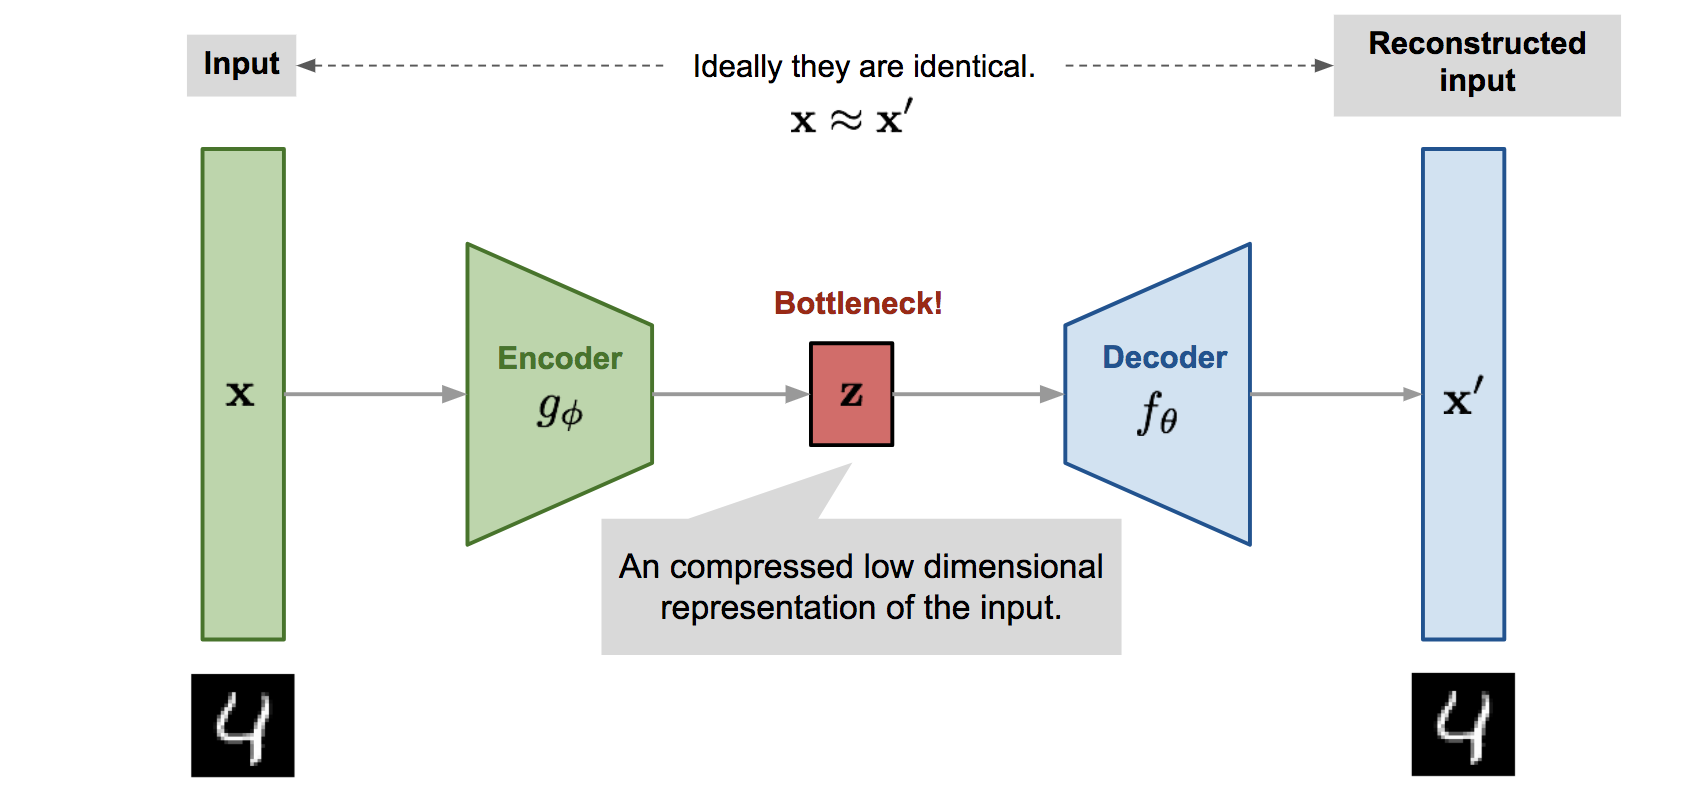
\includegraphics[width=\textwidth]{autoencoder-architecture}
\caption{We can think of this as a encoder (maximize by $\Phi$) and a decoder (maximize by $\theta$)}
\centering
\end{figure}
\\ \\ \\ \\ \\ \\ \\
We can look at the ELBO objective in another interesting way.\\
Let rewrite it to another formation :
\begin{gather*}
ELBO=\mathbb{E}_{z \sim q_{\Phi}(z)}[-log \ q_{\Phi}(z) + log \ p(z) + log \ p_{\theta}(X|z)] = \\ \\
= \underbrace{\mathbb{E}_{z \sim q_{\Phi}(z)}[log \ p_{\theta}(X|z)]}_{Reconstruction loss} - \underbrace{KL(q_{\Phi}(z|X)||p(z))}_{Regularization}
\end{gather*}
The reconstruction term assures that the model reconstructs $X$ accurately-how close is the input to the output. The regularization term adds regularization to the model preventing the NN model from overfitting the training data.\\
In order to prevent this, the regularization term keeps the distribution of the posterior simple. \\ \\

\section*{Optimization and representation trick}
The optimization problem that we saw above may be written:
\begin{gather*}
\underset{\theta, \Phi}{\arg\max} \ \mathbb{E}_{z \sim q_{\Phi}(z)}[f(z;\theta)] = \underset{\theta, \Phi}{\arg\max} \int_{z} q_{\Phi}(z)f(z;\theta)dz
\end{gather*}
Solving this problem requires the use of SGD or GD methods, which in turn need the derivatives. To find the derivatives we need to compute the integral, which are often hard to solve or intractable. We have seen that we can estimate the integral using Monte-Carlo approximation. However, using the Monte-Carlo approximation, removes the integrals dependency on $\Phi$ and thus we cannot find the derivative w.r.t $\Phi$ \\
To solve that we can rearrange the derivative w.r.t $\Phi$ :
\begin{gather*}
\nabla_{\Phi} (\mathbb{E}_{z \sim q_{\Phi}(z)}[f(z;\theta)]) =  \int_{z} \nabla_{\Phi}(q_{\Phi}(z))f(z;\theta)dz = \int_{z} \frac{q_{\Phi}(z)}{q_{\Phi}(z)}\nabla_{\Phi}(q_{\Phi}(z))f(z;\theta)dz = \\
= \int_{z} q_{\Phi}(z)\nabla_{\Phi}(log \ q_{\Phi}(z))f(z;\theta)dz = \mathbb{E}_{z \sim q_{\Phi}(z)}[\nabla_{\Phi}(log \ q_{\Phi}(z))f(z;\theta)] \approx \\ \approx \frac{1}{K}\sum_{k=1}^{K}\nabla_{\Phi}(log \ q_{\Phi}(z^{(k)})f(z;\theta)
\end{gather*}
This solves the above problem, but it turns out that this approximation is very noisy and requires many samples from $q_{\Phi}$. \\
To overcome this issue we can use the reparametrization trick : we choose $q_{\Phi} \sim N(\mu, \sigma^2)$ and then we using the normal distribution properties :
\begin{gather*}
\mathbb{E}_{z \sim q_{\Phi}(z)}[f(z;\theta)] = \mathbb{E}_{\epsilon \sim N(0,I)}[f(\mu_{\Phi} + \sigma_{\Phi}\epsilon;\theta)] \approx \frac{1}{K}\sum_{k=1}^{K}f(\mu_{\Phi} + \sigma_{\Phi}\epsilon^{(k)};\theta), \\ when \ \epsilon^{(k)} \sim N(0,I)
\end{gather*} 
Now to find an estimation for the derivative w.r.t $\Phi$. The parameters $\Phi$ are $\mu_{\Phi}, \ \sigma^2_{\Phi}$.
\begin{figure}[H]
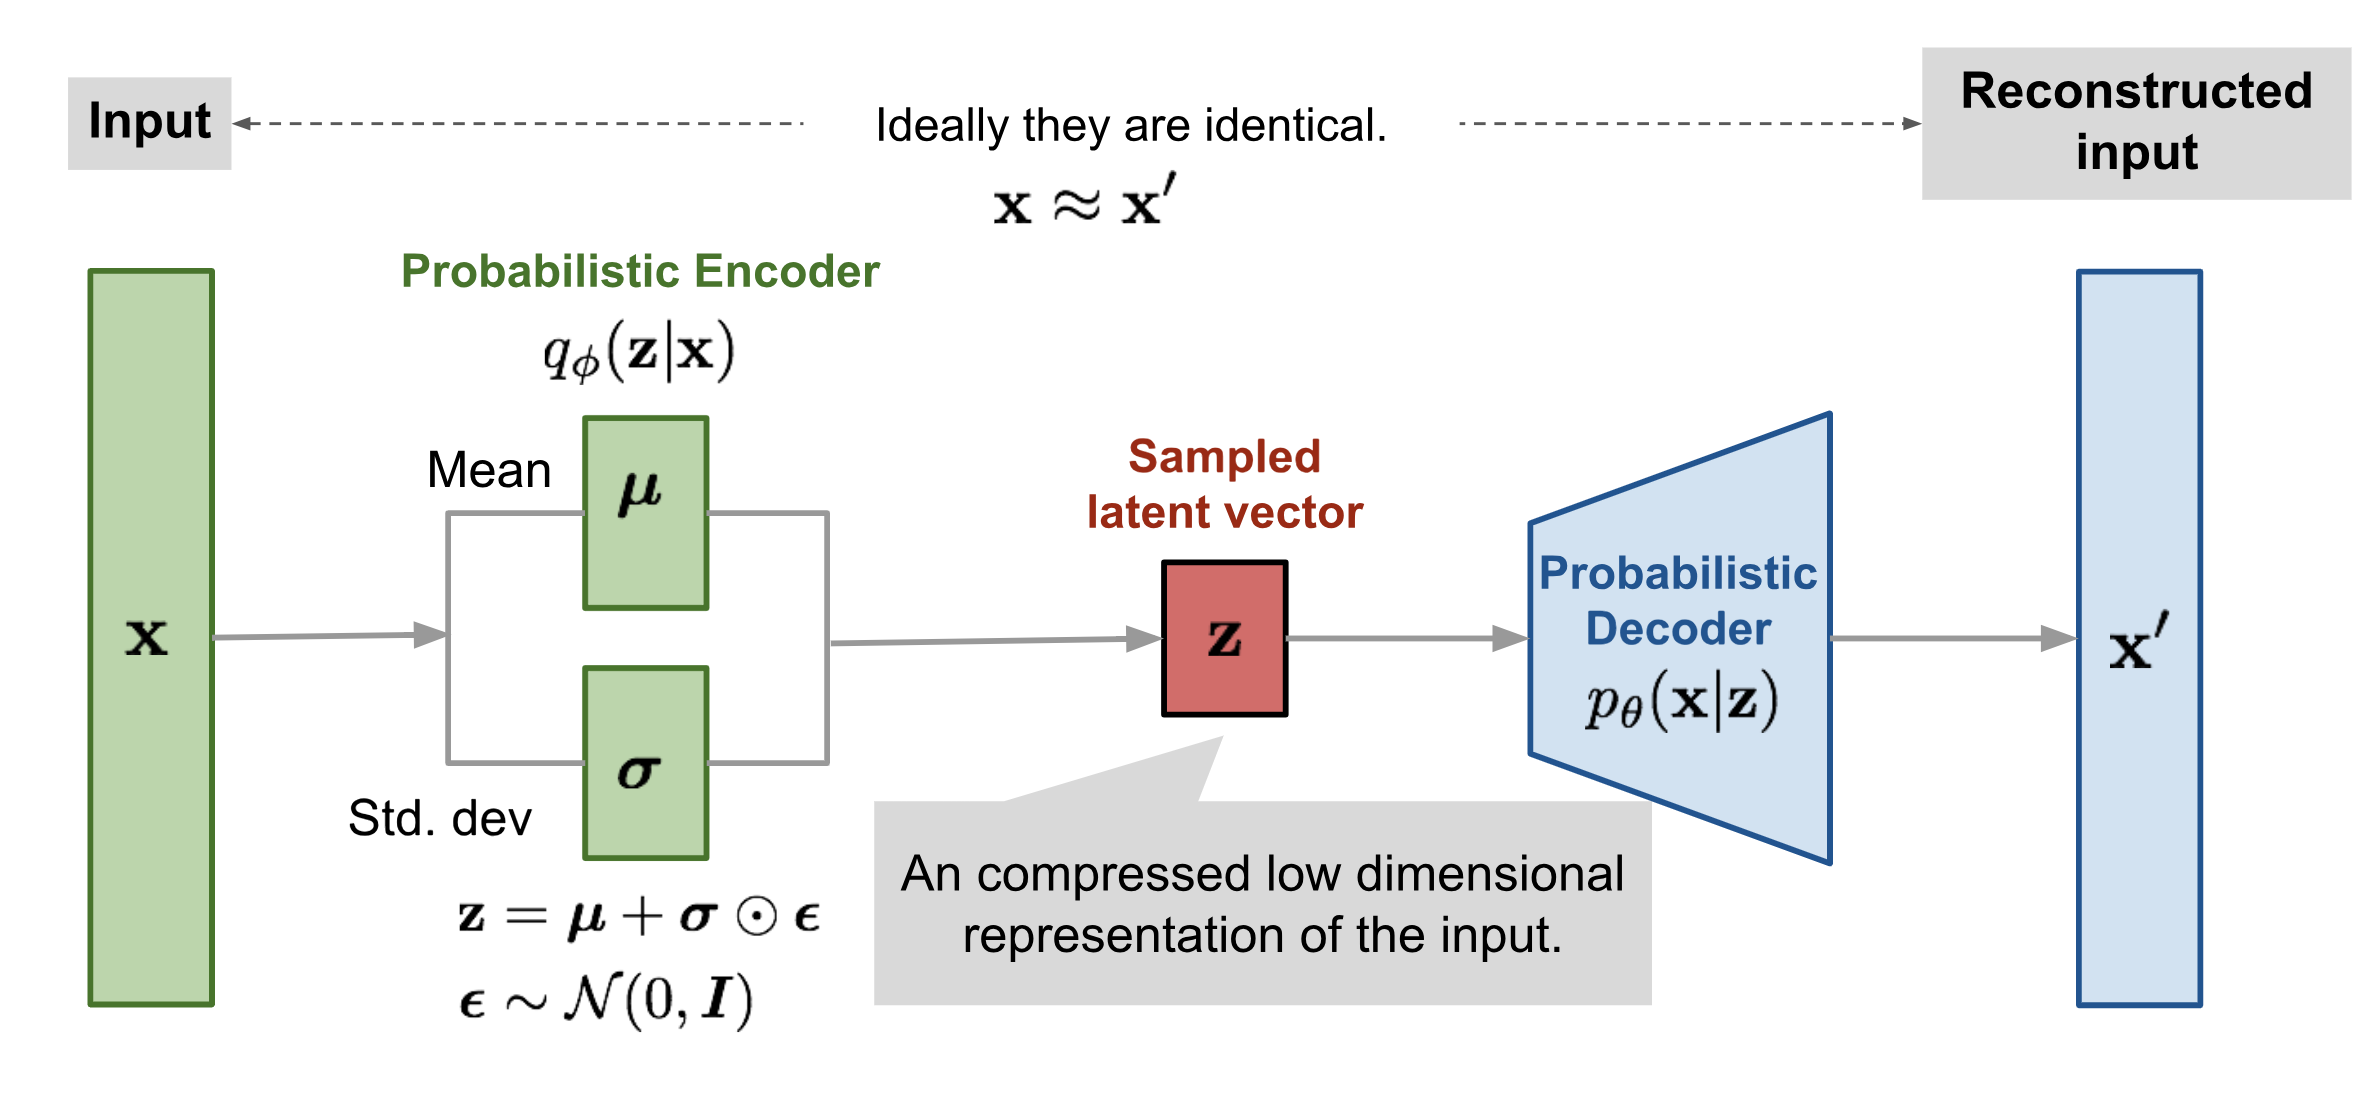
\includegraphics[width=\textwidth]{vae-gaussian}
\caption{To use the representation trick we just need to let $q_{\Phi}\sim N(0,I)$ and find an approximation to the derivative w.r.t $\Phi$ just by sample from the standard Gaussian}
\centering
\end{figure}
